\documentclass[UTF8]{ctexart}
%\documentclass{article}
\usepackage{graphicx,amsfonts,amsmath,mathrsfs,amssymb,amsthm,url,color}
\usepackage{fancyhdr,indentfirst,bm,enumerate,natbib, float,tikz,graphicx}
\usepackage{caption}
\usepackage{subcaption}
\usepackage{calligra} 

\title{微分方程概论2024期末回忆版}
\author{\textcalligra{NULIOUS}} 
\date{}

\textheight 23cm
\textwidth 16.5cm
\topmargin -1.2cm
\oddsidemargin 0cm
\evensidemargin 0cm

\begin{document}
\maketitle
\noindent 一.求解下列微分方程\\
1.$$x \frac{d y}{d x}=y-x \tan \frac{y}{x}$$
解:看到 $\tan \frac{y}{x}$ 自然想到作换元 $z=\frac{y}{x}$\\
并注意到 $\frac{d y}{d x} $,则$ x=0$ 不是解\\
两边除 $x$ ,并注意
$$
\frac{d y}{d x}=\frac{d(x z)}{d x}=x \frac{d z}{d x}+z$$
有
$$
\begin{aligned}
	\frac{d y}{d x}&=\frac{y}{x}-\tan \frac{y}{x}\\
 x \frac{d z}{d x}&=-\tan z\\
 \ln |\sin z|&+\ln |x|+c=0
\end{aligned}
$$
并取 $e$ 指数有通解 $$x \sin \frac{y}{x}=C^{\prime}$$\\


\noindent 2.$$y^{\prime}{ }^{\prime}+2 y^{\prime}+y=e^{-x}$$
解:这是高阶常系数线性方程,先求齐次通解\\
特征方程:$\lambda^{2}+2 \lambda+1=0 \Rightarrow \lambda=-1$(二重)\\
齐次通解:$$y=c_{1} e^{-x}+c_{2} x e^{-x}$$
对非齐次特解作待定系数 $\varphi(x)=a x^{2} e^{-x}$(注意 -1 是特征方程的二重根)
代入方程有 $a=\frac{1}{2}$ 。\\
通解:$$y=c_{1} e^{-x}+c_{2} x e^{-x}+\frac{x^{2} e^{-x}}{2}$$\\


\noindent 3.$$\sqrt{x} \frac{d z}{d x}+\sqrt{y} \frac{d z}{d y}=z$$
初值条件:$y=1$ 时,$z=\sin \pi x$\\
解:本题为 11.2 例 1 变式\\
$$\frac{d x}{\sqrt{x}}=\frac{d y}{\sqrt{y}}=\frac{d z}{z}$$
有独立首次积分:(需要用行列式检验独立性,在此不赘述)
$$
\left\{\begin{array}{l}
x-\sqrt{y}=c_{1} \\
2 \sqrt{y}-\ln |z|=c_{2}
\end{array}\right.
$$
隐式通解:$$\Phi(\sqrt{x}-\sqrt{y}, 2 \sqrt{y}-\ln |z|)=0$$
则
$$ z=\exp (2 \sqrt{y}) \varphi(\sqrt{x}-\sqrt{y})$$
其中 $\Phi, \varphi$ 为任意 $C^1$ 函数\\
代入初值 $$\sin \pi x=e^{2} \cdot \varphi(\sqrt{x}-1)$$
令 $\mathrm{k}=\sqrt{x}-1$ ,那么 $x=(1+\mathrm{k})^{2}$\\
$$\varphi(\mathrm{k})=e^{-2} \sin \left(\pi(1+\mathrm{k})^{2}\right)$$\\
最后
$$ z=e^{2 \sqrt{y}-2} \sin \left(\pi(1+\sqrt{x}-\sqrt{y})^{2}\right)$$\\


\noindent 4.求解 $$y^{3} d x+2\left(x^{2}-x y^{2}\right) d y=0$$
解:分组为 
$$\left(y^{3} d x-2 x y^{2}\right) d y+2 x^{2} d y=0$$
第一组积分因子为 $y^{-5}$ ,通积分为 $\frac{x}{y^{2}}=c$\\
第二组积分因子为 $x^{-2}$ ,通积分为 $2 y=c$\\
取 $$g_{1}(t)=t^{-2}\quad g_{2}(t)=2 t^{-1}$$ 
有 $$y^{-5} g_{1}\left(\frac{x}{y^{2}}\right)=x^{-2} g_{2}(2 y)$$ 
从而 
$$\mu=x^{-2} y^{-1}$$
同乘 $\mu$ 化简有 $$\ln y^{2}-\frac{y^{2}}{x}=c$$ 且 $y=0, x=0$ 为特解.\\


\noindent  二.求
$$
y=p^2-xp+\frac{x^2}{2} \quad p=\frac{dy}{dx}
$$
的通解和特解并画出其图像
解:两边对 $x$ 求导即可,可以写成因式分解的形式\\


\noindent 三.
\[
A=
\begin{pmatrix}
	2 & -1 & -1 \\
	-2 & 1 & 3 \\
	0 &-1 & 1 \\
\end{pmatrix}
\]
求其基解矩阵\\


\noindent 四.\\
1.画出 $\ddot{\theta}=5 \sin \pi \theta$ 的相图\\
解:这是二阶自治方程,作图请参考5.1节做法\\
令 $$v=\frac{d \theta}{d t} \quad \ddot{\theta}=\frac{d v}{d t}=\frac{d v}{d \theta} \frac{d \theta}{d t}=v \cdot \frac{d v}{d \theta}$$
则
$$v \cdot \frac{d v}{d \theta}=5 \sin \pi \theta$$
$$\Rightarrow v^{2}=-\frac{10}{\pi} \cos (\pi \theta)+C_{1}$$

\begin{figure}[h]  
	\centering  
	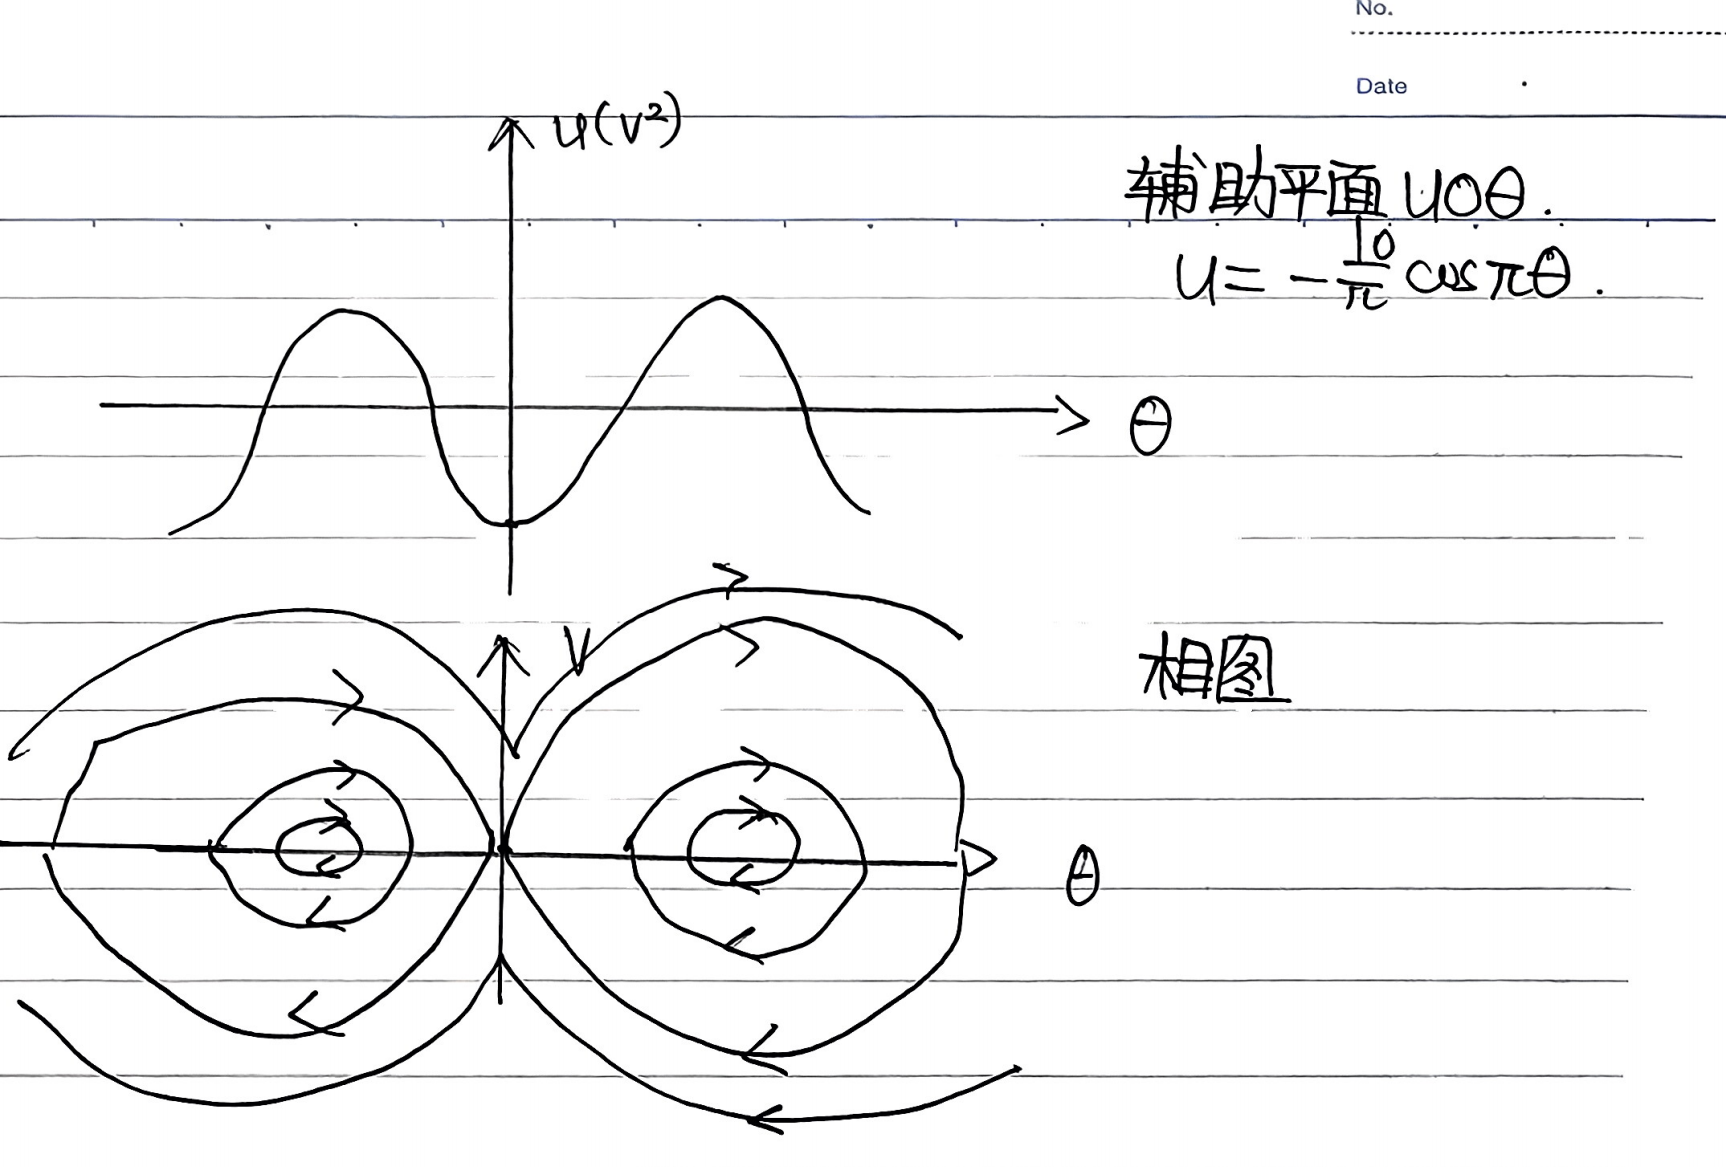
\includegraphics[height=5cm]{24期末.png} 
\end{figure}


\noindent 2.
\[
\begin{cases}
	\dfrac{d x}{d t}=x(2 y-1) \\ 
	\dfrac{d y}{d t}=y(3-4 x)
\end{cases}
\]
求此方程的一个在第一象限内的首次积分,并画出方程的相图\\
解:23年也考了这个方程\\
首次积分只需要将两式相除即可获得分离变量方程,注意题目要求在第一象限内\\
首次积分为 $$2 y-\ln y-3 \ln x+4 x=c$$
另外注意题目实际上已经给出了 $\frac{d\binom{x}{y}}{d t}=f(x, y)$ 的显式表达了,可以做出相图
\text{RK}:此题是洛特卡-沃尔泰拉的捕食者-猎物模型的一种情况\\


\noindent 五.判断下列方程解的稳定性\\
1.
\[
\left\{
\begin{array}{l}
	\displaystyle\frac{dx}{dt} =2x-y+x^2y+3y^2-5y^4\\ 
	\displaystyle\frac{dy}{dt} = x-y+x^2+2y^3
\end{array}
\right.
\]
解:注意到两个方程所含的项的个数并不相同,常规的李雅普诺夫函数无法用待定系数法凑出来,我们考虑线性近似,注意验证书上8.2.2给出的前提条件,发现满足要求,求一个二阶方阵的特征值即可\\


\noindent 2.
\[
\left\{
\begin{array}{l}
	\displaystyle\frac{dx}{dt} =-2\left(y^3+x^5 \right) \\ 
	\displaystyle\frac{dy}{dt} = x-y^3
\end{array}
\right.
\]
解:上下两个方程项数相等,仔细观察具体次方的不同,发现需要用 $V=a x^{2}+b y^{4}$ 来待定系数,求出 $a, b$ 即可\\
\textbf{RK}:一般情况下我们取 $V$ 的时候各取 $x$ 的一个偶数次方和 $y$ 的一个偶数次方待定系数\\


\noindent 六.\\
对下列方程的任意一个解,给出他的最大存在区间
$$
\frac{d y}{d x}=\left(2-y^{2}\right) e^{2\left(x^{2}+y^{2}\right)}
$$
解:仿照 23 年第三次习题课讲义的这道题即可\\
求证:初值问题
$$
\frac{d y}{d x}=(y-2 y-3) e^{(x+\mathrm{y})^{2}}, y\left(x_{0}\right)=y_{0}
$$
的解的存在区间为 $(a, b)$ ,则 $a=-\infty$ 或 $b=+\infty$ 至少存在一个.\\
Proof.注意到
$$
\left(y^{2}-2 y-3\right) e^{(x+y)^{2}}=(y-3)(y+1) e^{(x+y)^{2}}
$$
满足解的唯一性条件,且\\
(1)$y\equiv 3$ 与 $y \equiv -1$ 是两解\\
(2)$-1<y_{0}<3$ 时,解永远在 $-1<y<3$ 之间\\
(3)$y_{0}>3$ 时,此时解必满足 $y>3$ 成立( $y \equiv 3$ 为一解且过一点的解唯一),此时 $f(x, y)>0$ 恒成立,解向左延伸能延伸至负无穷。\\
(4)$y_{0}<-1$ 时,同理,$f(x, y)>0$ 会恒成立,向右延伸又不能越过 $y=-1$ .此时 $b=+\infty$ 。\\
对本题来说,虽然没有给出初值条件,但我们可以把通解中的常数 $C$看作"初值"来用相同的方法分析\\



\noindent 七.(本题 6 分)\\
方程 $$\quad \frac{d y}{d x}=f(x, y)$$
满足
$$
f(x, y)= \begin{cases}1, & (x, y) \neq(0,0) \\ 0, & (x, y)=(0,0)\end{cases}
$$
并且有解 $y=\varphi(x)$ 使得 $$\frac{d \varphi(x)}{d x}=f(x, \varphi(x))$$
求证:初值问题 $$\frac{d y}{d x}=f(x, y) ; y(0)=0$$
无解


\end{document}